\chapter[Projeto de Produtos e Serviços]{Projeto de Produtos e Serviços}
\label{chap:produtos}

	\section[Definição]{Definição}
	\label{sec:produtos_definicao}

		O objetivo que almeja-se alcançar ao projetar produtos e serviços é a satisfação dos consumidores, de maneira que suas necessidades e expectativas - atuais e/ou futuras – sejam atendidas. Praticamente todo projeto de produtos e serviços tem seu início e término com o consumidor. Primeiro, cabe a equipe de marketing buscar e compilar informações dos clientes (e, às vezes, de não-clientes) para compreender e identificar suas necessidades e expectativas e também para procurar possíveis oportunidades de mercado. 

		Com base nisso, a tarefa dos projetistas de produtos e serviços é analisar essas necessidades e expectativas, como interpretadas por marketing, e criar uma especificação para o produto ou serviço. Essa é uma tarefa complexa, que envolve a combinação de muitos aspectos diferentes dos objetivos operacionais de uma empresa. A especificação é então usada como informação de entrada para a operação, que produz e fornece o produto ou serviço a seus clientes. \cite{slack}

		\begin{figure}[h]
			\centering
			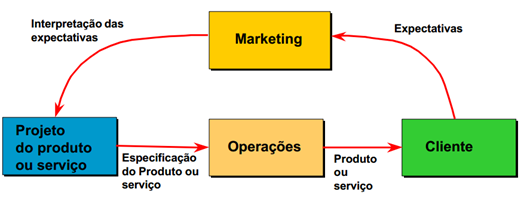
\includegraphics[scale=0.8]{produto1}
			\caption[Ciclo de realimentação cliente-marketing-projeto]{Ciclo de realimentação cliente-marketing-projeto.}
			\label{fig:produto1}
		\end{figure}

		Todavia, pode-se considerar que todos os produtos e serviços contam com três aspectos: 

		\begin{enumerate}
			\item{\textbf{Conceito} - Conjunto de benefícios esperados que o consumidor está comprando;}
			\item{\textbf{Pacote} - Conjunto de "componentes" que proporcionam os benefícios definidos no conceito;}
			\item{\textbf{Processo} - Define a relação entre os componentes dos produtos e serviços.}
		\end{enumerate}

		Tudo isso contribui e pode determinar se há um bom projeto de produtos e serviços. 

	\section[Etapas do Projeto]{Etapas do Projeto - \emph{Do Conceito à Especificação}}
	\label{sec:produtos_etapas}

		Para chegar ao ponto (conceito, produto, serviço), a atividade de projeto deve passar por diversas etapas. Essas formam uma sequência aproximada, embora na prática os projetistas geralmente circulem ou retrocedam pelas etapas. Serão descritas na ordem em que ocorrem usualmente.

		\begin{figure}[h]
			\centering
			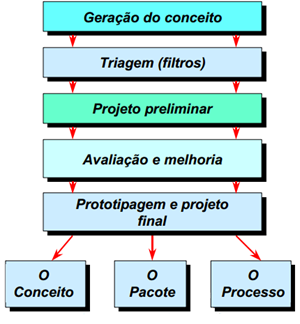
\includegraphics[scale=0.8]{produto2}
			\caption[Etapas do projeto do produto/serviço]{Etapas do projeto do produto/serviço.}
			\label{fig:produto2}
		\end{figure}

		\subsection[Geração do Conceito]{Geração do Conceito}
		\label{sec:produtos_etapas_geracaoConceito}

			Essa etapa inicia-se com ideias tanto de fontes externas quanto internas à organização, como dos consumidores a partir de grupos de foco, sugestões dos clientes e pesquisa de mercado, das ações dos concorrentes, dos funcionários e ideias da pesquisa e desenvolvimento. Essas ideias são transformadas no conceito do produto/serviço dando assim a forma, a função, o objetivo e os benefícios do produto/serviço de forma simplificada e de fácil entendimento.

		\subsection[Triagem]{Triagem}
		\label{sec:produtos_etapas_triagem}

			O conceito precisa ser aceito por toda a organização, sendo de essencial importância que ele passe por uma seleção (triagem) segundo os critérios de viabilidade (habilidade e capacidade produtivas), aceitabilidade (critérios satisfatórios) e vulnerabilidade (riscos) em cada uma das funções envolvidas, principalmente produção, marketing e finanças. Um projeto que leva em conta as qualificações da organização desde sua elaboração, é chamado por Stevenson (2001) de projeto voltado para as operações. 

		\subsection[Projeto Preliminar]{Projeto Preliminar}
		\label{sec:produtos_etapas_preliminar}

			Após a seleção do conceito do produto/serviço aceitável e consensual, este deve ser transformado em um projeto preliminar com as especificações dos produtos e serviços e a definição dos processos. Ou seja, especificam-se os componentes do pacote, a estrutura, isto é, a ordem na qual as partes componentes do pacote devem ser reunidas, a lista de materiais, as folhas de roteiro ou processo, as máquinas e equipamentos, os fluxogramas, os tempos e movimentos de todos os processos, as normas e procedimentos de execução, inspeção e controle e o arranjo físico. Além de, especificar o mercado consumidor, a previsão de demanda, a rede de suprimentos e os custos de produção. 

		\subsection[Avaliação e Melhoria]{Avaliação e Melhoria}
		\label{sec:produtos_etapas_avaliacaoMelhoria}

			O projeto preliminar será verificado para caso ele possa ser melhorado, em termos de utilização mais econômica e facilidade, antes de começar a ser produzido e posteriormente levado ao mercado, essa é a etapa de avaliação e melhoria do projeto. As técnicas mais utilizadas em avaliação e melhoria de projeto são: desdobramento da função qualidade - QFD (assegura o atendimento das necessidades dos clientes), engenharia de valor VE (reduz custos confrontando-os com as funções) e métodos de Taguchi (testa o desempenho do projeto diante de situações adversas).

		\subsection[Prototipagem e Projeto Final]{Prototipagem e Projeto Final}
		\label{sec:produtos_etapas_projetoFinal}

			Na última etapa do projeto, depois de avaliado e melhorado, ele é transformado em um protótipo para ser testado. Esses testes são realizados em cartão/papelão ou argila e simulações em computador com protótipos virtuais (CAD - projeto auxiliado por computador), usado para criar e modificar desenhos de produtos. Há também a possibilidade de fazer testes reais com os consumidores em escala-piloto. 
            
            Dentro desse contexto global e competitivo, revela-se a importância da elaboração do projeto de produtos e serviços, que desde os aspectos iniciais da geração do conceito até o produto final e assistência ao cliente deve nortear as organizações. 


    	Verifica-se a partir do estudo realizado que as organizações necessitam de bons projetos para angariar cada vez mais consumidores. Pois, a criação de produtos que atendam às necessidades desses, pode por ventura ser o ponto de partida para estabelecer uma vantagem competitiva, e consequentemente será conseguido o sucesso estratégico da empresa.

	\section[Aplicações]{Aplicações - 
\includegraphics{bobs2}}
	\label{sec:produtos_aplicacoes}

		Como visto na parte de Projeto de Processos, o \textbf{Bob’s} se enquadra em um projeto de serviços, de acordo com a definição do \cite{slack}. Serviços estes que baseavam-se em 3 diretrizes: sempre a \textbf{melhor qualidade} no \textbf{produto} e na \textbf{limpeza}. Com o tempo toda marca sofre melhorias e aprimoramentos, sempre levando em conta a sua identidade. Identidade esta que é reforçada pelo conceito da marca. 

		Quando se entra em uma unidade \textbf{Bob’s} é notória a preocupação quanto à saúde de todos, especialmente com o público infantil. Existe uma política especial para esse público. Não há publicidade de alimentos ou bebidas para crianças abaixo de 12 anos, exceto com produtos cujo perfil nutricional atenda a critérios específicos baseados em evidências científicas. Hoje a rede \textbf{Bob’s} acredita que a responsabilidade social, a ética, a preservação do meio ambiente e a valorização dos seus funcionários são valores essenciais para o seu crescimento. Para o \textbf{Bob’s} a sua responsabilidade com a sociedade se inicia com o respeito ao público interno, dando ótimas condições de trabalho e ainda em um ambiente agradável, resultando em equipes motivadas e produtivas.

		Todo esse conceito é o que a rede \textbf{Bob’s} quer passar a seus clientes, desde a criança ao idoso. Inclusive por meio de políticas que respeitam esse público. Sendo por exemplo, a primeira empresa \emph{“fast food”} em contratar profissionais da terceira idade, trocando experiências entre seus colaboradores do Projeto Melhor Idade e os jovens que ingressaram pelo programa Primeiro Emprego. Tudo isso por se preocupar com o cliente.

		A rede \textbf{Bob’s} oferece seus serviços por meio de uma rede compostas de: lanchonetes, quiosques, Drive Thru e um serviço especial de entrega, \textbf{Bob’s \emph{Delivery}}. O \textbf{Bob’s} com a imagem que a maioria das pessoas conhecem surgiu em 2002, com uma estratégica redefinição. Com cardápio incrementado com novos itens e novas lojas inauguradas, os gestores decidiram cuidar da imagem da rede e do design das lojas. Comemorado em 2002, 50 anos, lançou-se o sexto logotipo da rede, o primeiro desde a fundação a ter três cores (vermelho, azul e amarelo), em vez de duas (branco e vermelho). 

		As lojas antigas ganharam letreiros coloridos e um mobiliário mais moderno. As novas lojas, por sua vez, passaram a ser mais compactas e aconchegantes. Com essas mudanças, o \textbf{Bob’s} Original, como era chamado, a rede voltou a vender sanduíches que marcaram época e hoje não existem mais no cardápio da rede, como o de salada de ovo, além dos hambúrgueres feitos e servidos numa frigideira.

		Novos conceitos de ponto-de-venda também forma introduzidos: os chamados quiosques, que têm, em média, apenas $15 m^2$ e são destinados aos corredores de shopping centers e aeroportos, e o da mini-loja, uma unidade móvel produzida em aço galvanizado, de $23 m^2$ para ser instalada em ruas, estacionamentos de hipermercados e praças públicas. Criou um formato especial para suas unidades exclusivas de sobremesas geladas, o \textbf{Bob’s \emph{Shakes}}, investiu no cardápio de café da manhã e mais recentemente ampliou a linha de hambúrgueres de picanha com três novas combinações. Hoje já são 1,1 mil lojas espalhadas pelas principais cidades do país. \cite{lamonica}

		Neste ano, a rede anunciou uma nova estratégia de marketing, que incluiu a apresentação de uma nova identidade visual (logotipo e embalagens), a renovação do cardápio, com novos ingredientes e até diferentes tamanhos de lanches, além de uma total renovação do ambiente de suas lojas, que será efetuada aos poucos. As novas unidades, além de um \emph{layout} mais moderno, contam com autosserviço de bebidas, possibilidade de personalização de produtos, molho à vontade e sanduíches em tamanhos P, M e G. Outra mudança que deve fazer muito sucesso neste novo conceito é o pedido “no capricho”, que permite ao consumidor aumentar a quantidade de um ingrediente de seu sanduíche - exceto carne e pão - sem nenhuma cobrança adicional.

		Tudo isso para atender melhor o cliente. Servindo pratos totalmente adaptados ao paladar brasileiro. Mas, para chegar a esse resultado, foi preciso passar pela opinião do consumidor, dos empregados, etc. Foi preciso enfrentar cada uma das etapas de projeto. Ter uma forte equipe de marketing, o que levou a equipe definir novas combinações de produtos. Até mesmo o fato de estar presente em todos os estados brasileiros. 

		A empresa, além de disponibilizar seu cardápio, juntamente com suas promoções, oferece suas opções de \emph{delivery}, que pode ser realizado via telefone, computador e mobile por meio de um aplicativo, fazendo da internet um forte aliado para atrair clientes de várias faixas etárias. 